\documentclass[11pt]{article}
% \usepackage[french]{babel}
%  \usepackage{DejaVuSans}
%  \usepackage{libertine}
%  \renewcommand*\rmdefault{cmfib} 
% \usepackage[default]{cantarell}

% \usepackage[T1]{fontenc}
% \renewcommand{\rmdefault}{cmss}  
% \fontencoding{T1}
%   \fontfamily{cmss}
%   \fontseries{m}
%   \fontshape{n}
%   \fontsize{10}{15}
% \renewcommand*\familydefault{cmss}
%   \selectfont
% \usepackage[utf8]{inputenc} 
\usepackage{array, xcolor, lipsum, bibentry}
\usepackage[top=1.6cm, bottom=1.5cm, left=1.8cm, right=1.9cm]{geometry} 
% \usepackage[margin=2.0cm]{geometry} 
%lmargin=3.0cm, rmargin=1.0cm,tmargin=2.50cm,bmargin=2.50cm
\usepackage{longtable}
\usepackage{fancyheadings}
 \pagestyle{fancyplain}
 \fancyhead{}
\fancyfoot{}
\renewcommand{\headrulewidth}{0pt}
\cfoot{\thepage}
\rfoot{\scriptsize \selectfont Iliya Enchev \longdate{\today}}
% \usepackage{helvet}
% \usepackage[french]{babel}
% \usepackage[T1]{fontenc}
% \usepackage[utf8]{inputenc}

% \usepackage[T1]{fontenc}
\usepackage{graphicx}
\usepackage[light,math]{iwona} 
% \usepackage{DejaVuSans}
%   \renewcommand{\rmdefault}{cmss}  
%   \renewcommand{\sfdefault}{cmr}
%   \renewcommand{\ttdefault}{ptm}

%     \usepackage{titlesec}
%     \titleformat{\section}{\large\bfseries}{\thesection}{1em}{}
 
\newcommand{\addphoto}[2]{%
  \smash{%
    \makebox[0pt][l]{%
      \raisebox{#1pt}{%
        \hspace{#2pt}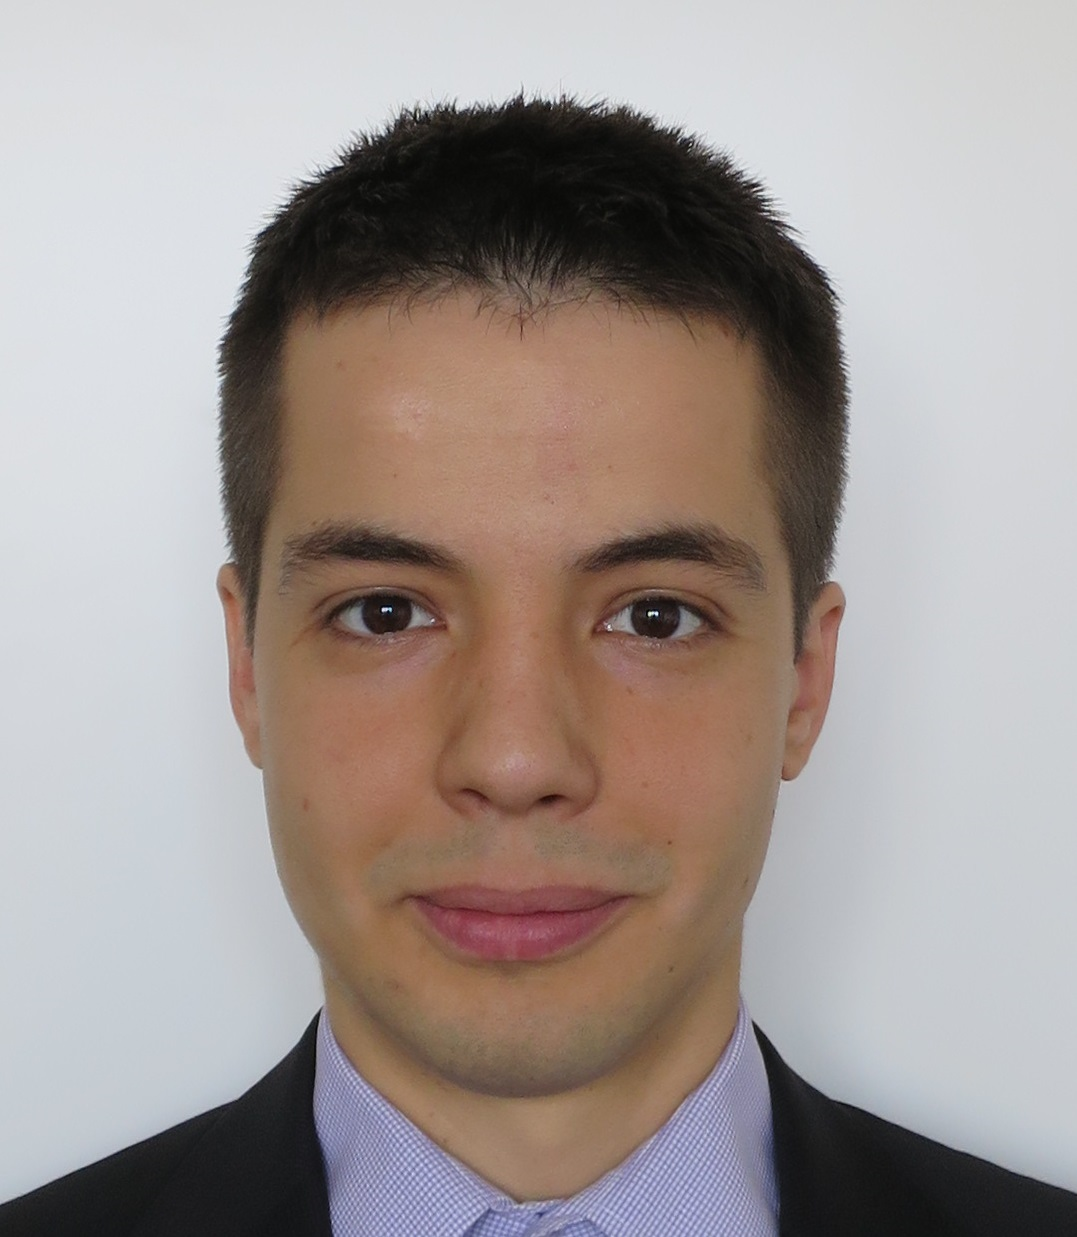
\includegraphics[width=3.4cm]{iliya_mug_0715}%IMG_9061cropped3
        % bgMasterPhotoSmall
%         \includegraphics[width=3.7cm]
        % PersonalFotoBgMaster
      }%
     }%
  }%
}

%ptm phv pcr 
% \renewcommand{\rmdefault}{iwona}
% \renewcommand{\sfdefault}{iwona}
\usepackage[nodayofweek]{datetime}
\title{\bfseries\huge Iliya Stefanov Enchev\\
\addphoto{10}{138}}
\author{iliyastefanov@gmail.com}
\date{\today}
% \addphoto{5}{150}

\definecolor{lightgray}{gray}{0.8} 
\newcolumntype{L}{>{\raggedleft}p{0.20\textwidth}}
\newcolumntype{R}{>{\arraybackslash}p{0.75\textwidth}X}
\newcommand\VRule{\color{lightgray}\vrule width 0.5pt}


% \begin{filecontents}{publication.bib}
% @article{lamport1986latex,
%   title={LaTEX: User's Guide \&amp; Reference Manual},
%   author={Lamport, L.},
%   year={1986},
%   publisher={Addison-Wesley}
% }
% @book{knuth2006art,
%   title={The art of computer programming: Generating all trees: history of combinatorial generation},
%   author={Knuth, D.E.},
%   volume={4},
%   year={2006},
%   publisher={addison-Wesley}
% }
% \end{filecontents} 

\begin{document}
% \addphoto{5}{150}


% 
\includegraphics{picture.jpg}
% \normalfont
% \maketitle
% \vspace{0.5em}
\section*{}
 
\begin{minipage}[ht]{0.68\textwidth} 
{\bfseries\huge Iliya Stefanov Enchev}\\
\newline
%iliyastefanov@gmail.com\\
iliyastefanov@gmail.com\\
+41 77 43 777 03\\
Rue Aloys-Mooser 3\\
1700 Fribourg\\
Switzerland\\
%Nationality: Bulgarian\\
% \formatdate{}{}{1986} 
Born: 29.03.1986
\end{minipage}
\begin{minipage}[ht]{0.48\textwidth}
% Nonlandian\\
% January 3rd, 2020\\
% +12 34 56 789

\addphoto{-111}{57}
% ~
% ~
% ~
% \newline
% \vspace{-15mm}
\vspace{112pt}  
\hspace{19mm} \longdate{\today}
\end{minipage}
\vspace{1pt}
%15pt



%Find a job as a spaceship commander!

\section*{Relevant work experience}

\begin{tabular}{L!{\VRule}R}
Docuteam GmbH\\
{\bf Software Engineer}\\
Mar. 16--Sept.16&Maintenance and development of in-house Java tools,
bug fixing, Continuous Integration and coding and design standards proponent.\\
Acquired skills\\&Java 7,8, JUnit, Ant, Maven, Nexus, Archival Standards.\\
ELCA Bern\\
{\bf DWH/ETL Developer}\\
Jun. 14--Jul.15&{\it Consultant by CFF} with several ETL projects. Development
of a Java application for automated Host DB2 to Oracle migration, DDL scripts,
automated workflow loading and running; bitemporal, analytical and hierarchical
queries; ETL platform admin.\\

Acquired skills\\&PowerCenter ecosystem,
DWH/ETL, Oracle SQL, Unix, Bash, Java, Maven, Regex.\\
{\bf Software Engineer}\\
Oct. 13--May 14&{\it ASTRA Road Traffic Management} --
%for the Federal Roads Office. 
Development of new features - from web service
consumption or DB access up the stack to the UI, bug fixing and testing.\\

Acquired skills\\&Java, GWTP, GXT, Hibernate, Spring, Maven, Continuous
Integration (Jenkins), JUnit.\\
%\\&\\

% LDBC\\
% {\bf Dissemination Mgr}\\
% Oct. 14 -- Mar. 15\\&Part-time, helped the dissemination efforts of the European
% funded project Linked Data Benchmark Council. Took part in the writing of
% several blog posts, was responsible for social media accounts. Achieved several
% peaks in activity.\\

% Developed several new features of the application from web service consumption or DB access up the
% stack to the UI. Applied a JavaScript library for time series visualisation,
% partisipated in bug fixing and performance testing.
%Bug fixing including a bug with unecessary rebuild of UI that hampered
%performance. 
%Acquired knowledge in: Java, GWTP, GXT, Hibernate, Spring, Maven, Continuous
% Integration (Jenkins), JUnit, etc.\\

eXascale Infolab by Prof. Cudr\'e-Mauroux\\
{\bf Scientific Collaborator}\\
Jan. 11--May 13\\&{\it NoSQL RDF Benchmark} -- Implemented a SPARQL endpoint
with Apache Jena and a NoSQL database for cluster benchmarking. \cite{nosqlrdf}
%running benchmark
%tests on clusters of up to 16 nodes. 
% Implemented a SPARQL endpoint with Apache
% Jena on top of Couchbase document database for running Berlin and
% DBpedia SPARQL Benchmarks on clusters of up to 16 nodes with large
%datasets.
{\it Project Bowlogna} -- Transformed relational
university data into RDF ontology and developed a web visualization for
interaction with it. Developed ontology generator based on the same data. \cite{
bowlognaBench, bowlFost}
% Technologies: Java, Hibernate, Jena, AllegroGraph, SPARQL, JavaScript, Ajax,
% jQuery.

Java, CouchBase, Unix,
SPARQL, Hibernate, AllegroGraph, JavaScript, Ajax, jQuery,
collaborative scientific writing.\\
\\
%\end{tabular}
%\begin{tabular}{L!{\VRule}R}
DERI, Ireland\\
{\bf Intern}\\
%supervised by Michael Hausenblas\\
Nov. 12--Feb. 13\\
&{\it Project Spitfire, LD4Sensors} -- IOT application for enriching sensor
observations and metadata with Linked Data.
%Decoupled the underlying RDF store
%from the Linked Data annotations layer, so data can be modified by other
%applications, improved the application's REST API.

Java, Git, Maven, REST.\\


%\end{tabular}

%\begin{tabular}{L!{\VRule}R}
% Jan. 11--May. 12&{\bf Collaborator at University of Fribourg}, Switzerland \\
% &{\it Project Bowlogna}--an application for generating ontologies of
% customizable size, based on real data from the Faculty of
% Humanities. Transforming relational university data into RDF ontology and
% developing a Web visualisation for interaction with it, using Jena,
% AllegroGraph, SPARQL, JavaScript, Ajax, jQuery, Cytoscape
% Web.\cite{ bowlognaBench, bowlFost}\\

%\end{tabular}

%\clearpage
%\section*{}
%\begin{tabular}{L!{\VRule}R}
Musala Soft, Bulgaria\\
{\bf Junior Software Engineer}\\
Feb. 09--Aug. 10&Two Java EE Projects focused on development and testing. One
data integration project focused on SQL, PL/SQL, refactoring.

Java EE, Hibernate, Oracle DB, SQL, JSF, EJB 3.0, Web
Services, Agile Methodologies, communication in large distributed teams. SCJP Certificate.
 %Experience with  {\it
%Barracuda for Mtel} --
%The biggest mobile operator in Bulgaria, part of Mobilkom Austria Group. 
%Integration project for substituting legacy
%billing%, ordering 
%and CRM systems.
%  with products developed by Amdocs.\\
%{\it Declaration Management System (DMS)} with IBM Netherlands -- 
%control and administation of movements
%of goods through Dutch Customs.

%{\it Content Delivery Platform} for Mobilkom Austria, 
%application for mobile entertainment content, % on mobile phones 
% -- games, ring tones, pictures 
%accessible through Web or WAP interface.

%Responsible for refactoring and testing PL/SQL procedures that extract
%information relevant to billing cycles and different kinds of services and 
%subscribers and provide this information to SAP 
%accounting system. Code design, implementation and refactoring. 
%integration activities, close communication with team members, troubleshooting
%critical production issues. 
%Technologies: Java EE, JSF, EJB, Hibernate ORM, Oracle DB.\\
\end{tabular}

%\section*{IT Skills}
%\begin{tabular}{L!{\VRule}R}
%software development&Java SE/EE, JSP, JSF, Servlets,
%Hibernate, JavaScript, JSON, Ajax, jQuery, Web Services, Oracle DB, SQL,
% PL/SQL, Apache Cassandra, Couchbase, MapReduce, RDF, Apache Jena, SPARQL, Linux, Git, SVN
%\\
% \end{tabular}
% 
% \section*{}
% \begin{tabular}{L!{\VRule}R}
% tools&dsdad\\
% certification&Sun Certified Programmer for the Java Platform, Standard Edition 6\\
% &Sun Certified Business Component Developer for the Java EE 5\\
% \end{tabular}

% \section*{Master's thesis}
% \begin{tabular}{L!{\VRule}R}
% title&{\bf Unconventional Store Systems for RDF Data} \\
% supervisor&Prof. Philippe Cudr�-Mauroux\\
% description&Overview of some main points of the Web, Semantic Web and Linked Data. Presenting a number of registry
% systems that handle data broadly generalized as entities with identifiers -- DNS, DOA, ENS, Chord DHT and CoralCDN. 
% Comparison of four data storage solutions -- AllegroGraph, Open Chord, Apache
% Cassandra, MySQL in their ability to handle RDF entities, using a benchmarking
% suite developed in Java.\cite{downScale}
% \end{tabular}

\section*{Education}
\begin{tabular}{L!{\VRule}R}

%Presenting a number of registry systems that handle data broadly generalized
%as entities with identifiers -- DNS, DOA, ENS, Chord DHT and CoralCDN.
%Comparison of four data store solutions -- AllegroGraph, Open Chord, Apache
%Cassandra, MySQL in their ability to handle RDF entities, using a benchmarking
%suite developed in Java.\cite{downScale}\\
BeNeFri\\
{\bf MSc in Computer Science}\\
Sep. 10--Oct. 12&
% Science in Computer Science, Universities of Fribourg, Bern and Neuch\^atel,
% Switzerland\\ %\vspace{5pt}

Master's thesis: {\bf Unconventional Store Systems for RDF Data},
overview on main points of the Web, Semantic Web and Linked
Data. Analysis and performance comparison of data store and entity registry
systems -- {\bf DNS}, DOA, ENS, Chord DHT, CoralCDN, AllegroGraph, {\bfApache
Cassandra} and MySQL in their ability to handle RDF entities, using own Java benchmarking suite.\cite{downScale}
During studies: emphasis on Software Engineering -- several courses on
Concurrent programming, Agile Methodologies, Data Management, Ubiquitous
computing, Distributed Systems, User Centered Desing; three projects based on
GWT, Google maps API, SOAP, REST, MongoDB. \\
\\
% Django; \\
{\bf BSc in Computer Science}\\
2005--2009&German Engineering Faculty of the
Technical University of Sofia, Bulgaria; courses taught in German\\
Mar. 08--Aug. 08&Erasmus exchange student, Karlsruhe Institute of
Technology -- KIT, Germany\\
\\
{\bf Languages}&Bulgarian (Macedonian), English, German, French, Russian
% {\bf Languages}&Bulkgarian (mother tongue), English, German, French, Russian
 \end{tabular}

 
\section*{Miscellaneous}
\begin{tabular}{L!{\VRule}R}
Leisure&Cooking, cycling, bicycle reparation, singing, 
% playing a %Bulgarian folk instrument -- gadulka; 
travelling, Drupal website\\
%all sorts of bikes;
%swimming; 
%playing a Bulgarian folk instrument -- gadulka; travelling locally and %since
% elementary school
%abroad; cooking \\
%soft skills&social networks, online hangouts for open source projects; a good
%team player\\
Driver's license&A+B since 2004\\
\end{tabular}

    %\renewcommand\bibsection{\subsection{\refname}}
    
\renewcommand{\refname}{Publications}
\begingroup
    \fontsize{9pt}{11pt}\selectfont
\bibliographystyle{abbrv}%alpha plain abbrv
% \nobibliography{publication}

\bibliography{publication}
   %\renewcommand\@biblabel[1]{\textbullet}
% \nocite{*}
\endgroup
% \section*{Publications} 
\fontsize{14pt}{0pt}
%\selectfont
% \resizebox{\textwidth}{!}{
% \begin{tabular}{L!{\VRule}R} 
%\bibentry{downScale}
%\newline
%\bibentry{bowlFost} %\vspace{5pt} 
%\newline
%\bibentry{bowlognaBench}
% \end{tabular} 
%{%\vspace{20pt}\newline
% \vspace{5pt}
% \newline
% \newline
% \newline
% \vspace{5pt}
% \newline
%\vspace{35pt}
%\scriptsize\hfill Iliya Enchev \longdate{\today}} 
\end{document}